\chapter{設計}
\label{chap:sekkei}

本章ではハイパーイラストと手書きベースWikiの要件と設計について述べる。

\newpage

\section{要件}
前章で示した画像ファイルフォーマットや手書きデータを扱う既存のツールの問題点を踏まえて、本システムの要件を整理する。
\begin{enumerate}
    \item 簡単に手書きメモのメモやイラストが作成・編集できる\\
    気軽に手書きメモ・イラストを取ることができ、また再編集性も可能である。
    \item 作成した手書きのメモやイラストを簡単に参照したり、再利用したりできる\\
    画像の内部に対してハイパーリンクを設定でき、関連する画像を参照することができる。
\end{enumerate}
これらの要件を満たすシステムは次世代の画像ファイルフォーマットであるハイパーイラストと、その作成・編集と管理をサポートする手書きベースWikiの組み合わせによって実現可能である。

\section{ハイパーイラスト}
本研究ではハイパーテキストの特徴を取り入れることによって既存の画像ファイルフォーマットの問題点を解決する
ハイパーイラストを提案する。

\subsection{ハイパーイラストの定義}
\begin{itemize}
    \item テキストではなく手書きによって記述される \\
    HTML等のハイパーテキストは記法に基づいたテキストによってマークアップされるが、
    ハイパーイラストはタッチやスタイラスから取得される手書きデータによってその内容が記述される。
    \item 内部の任意の要素にハイパーリンクが埋め込むことができる \\
    ハイパーテキストがその内部に他の文書への参照を示すハイパーリンクを埋め込むことができるように、
    ハイパーイラストは内部にハイパーリンクを埋め込むことができる。
\end{itemize}

\begin{figure}[htbp]
    \begin{center}
    {
\includegraphics[width=50mm]{images/testimage.png}} \end{center}
    \caption{ハイパーイラストの概念図}
\end{figure}

\subsection{ハイパーイラストの仕様}
本研究におけるハイパーイラストはSVG\cite{aboutsvg}というフォーマットをベースとしている。
SVGはXML\footnote{https://www.w3.org/XML/}をベースとしており、他の画像ファイルフォーマットにはない、ハイパーイラストに適した以下のような特徴を持つ。
\begin{itemize}
    \item グラフィカルな表現を前提に設計されている
    SVGには曲線等を表現するPath要素や閉じた図形を表現するPolygon要素等の仕様が標準で備わっている。
    スタイラスから得られるデータをPath要素の属性として定義することで手書きのストロークを表現することができる。
    \item 構造を保持できる\\
    ラスターイメージと異なりSVGの実体は構造化されたテキストファイルであり、線分や点はピクセルではなく
    独立した要素として記述される。これにより書き順等の構造も保持され、再編集性が高い。
    \item ハイパーリンクを埋め込める\\
    SVGではXLink\footnote{https://www.w3.org/TR/xlink/}形式のハイパーリンクを任意の要素に埋め込むことができるため
    画像の中の個別の要素に対して複数のリンクを定義することができる。
    \item Web標準の技術である\\
    SVGは特定の企業の製品ではなく、その仕様は全て公開されている。また作成や表示に特別なソフトウェアを必要とせず、
    ブラウザのみで閲覧することができる。
\end{itemize}

\section{手書きベースWiki}
%本研究で提案する手書きベースWikiの基本構成及び使い方を解説する。
%既存のテキストベースWikiがテキスト入力によって作成されたハイパーテキストをコンテンツとするように、
%手書きベースWikiでは手書き入力によって作成されたハイパーイラストをコンテンツとして管理する。
ハイパーイラストをコンテンツとするWikiシステムである手書きベースWikiも提案する。


\subsection{手書きベースWikiの定義}
\begin{itemize}
    \item ハイパーイラストを作成・編集できる\\
    タッチやスタイラスに対応したエディタを備え、手書きによって
    ハイパーイラストを手軽に作成・編集することができる。
    \item ハイパーイラストにハイパーリンクを追加できる \\
    作成したハイパーイラスト同士の相互リンクを簡単な操作で定義できる。
    \item 関連するハイパーイラストを参照できる \\
    ハイパーイラスト同士のリンク関係を元に、関連するハイパーイラストを
    一覧できるよう表示する。
\end{itemize}
この要件を満たす手書きベースWikiのプロトタイプしてDrawWikiを開発した。

\subsection{DrawWiki}
DrawWikiは本研究において開発した、手書きベースWikiのコンセプトを元にしたプロトタイプとなるアプリケーションである。(図\ref{drawwiki})
%手書きベースWikiはハイパーイラストを作成・編集する手書きエディタと、
%作成したハイパーイラストやそれに関連するハイパーイラストを参照・表示する部分にわかれている。
本章ではその主要な機能を使い方とともに解説する。

\begin{figure}[htbp]
    \begin{center}
    {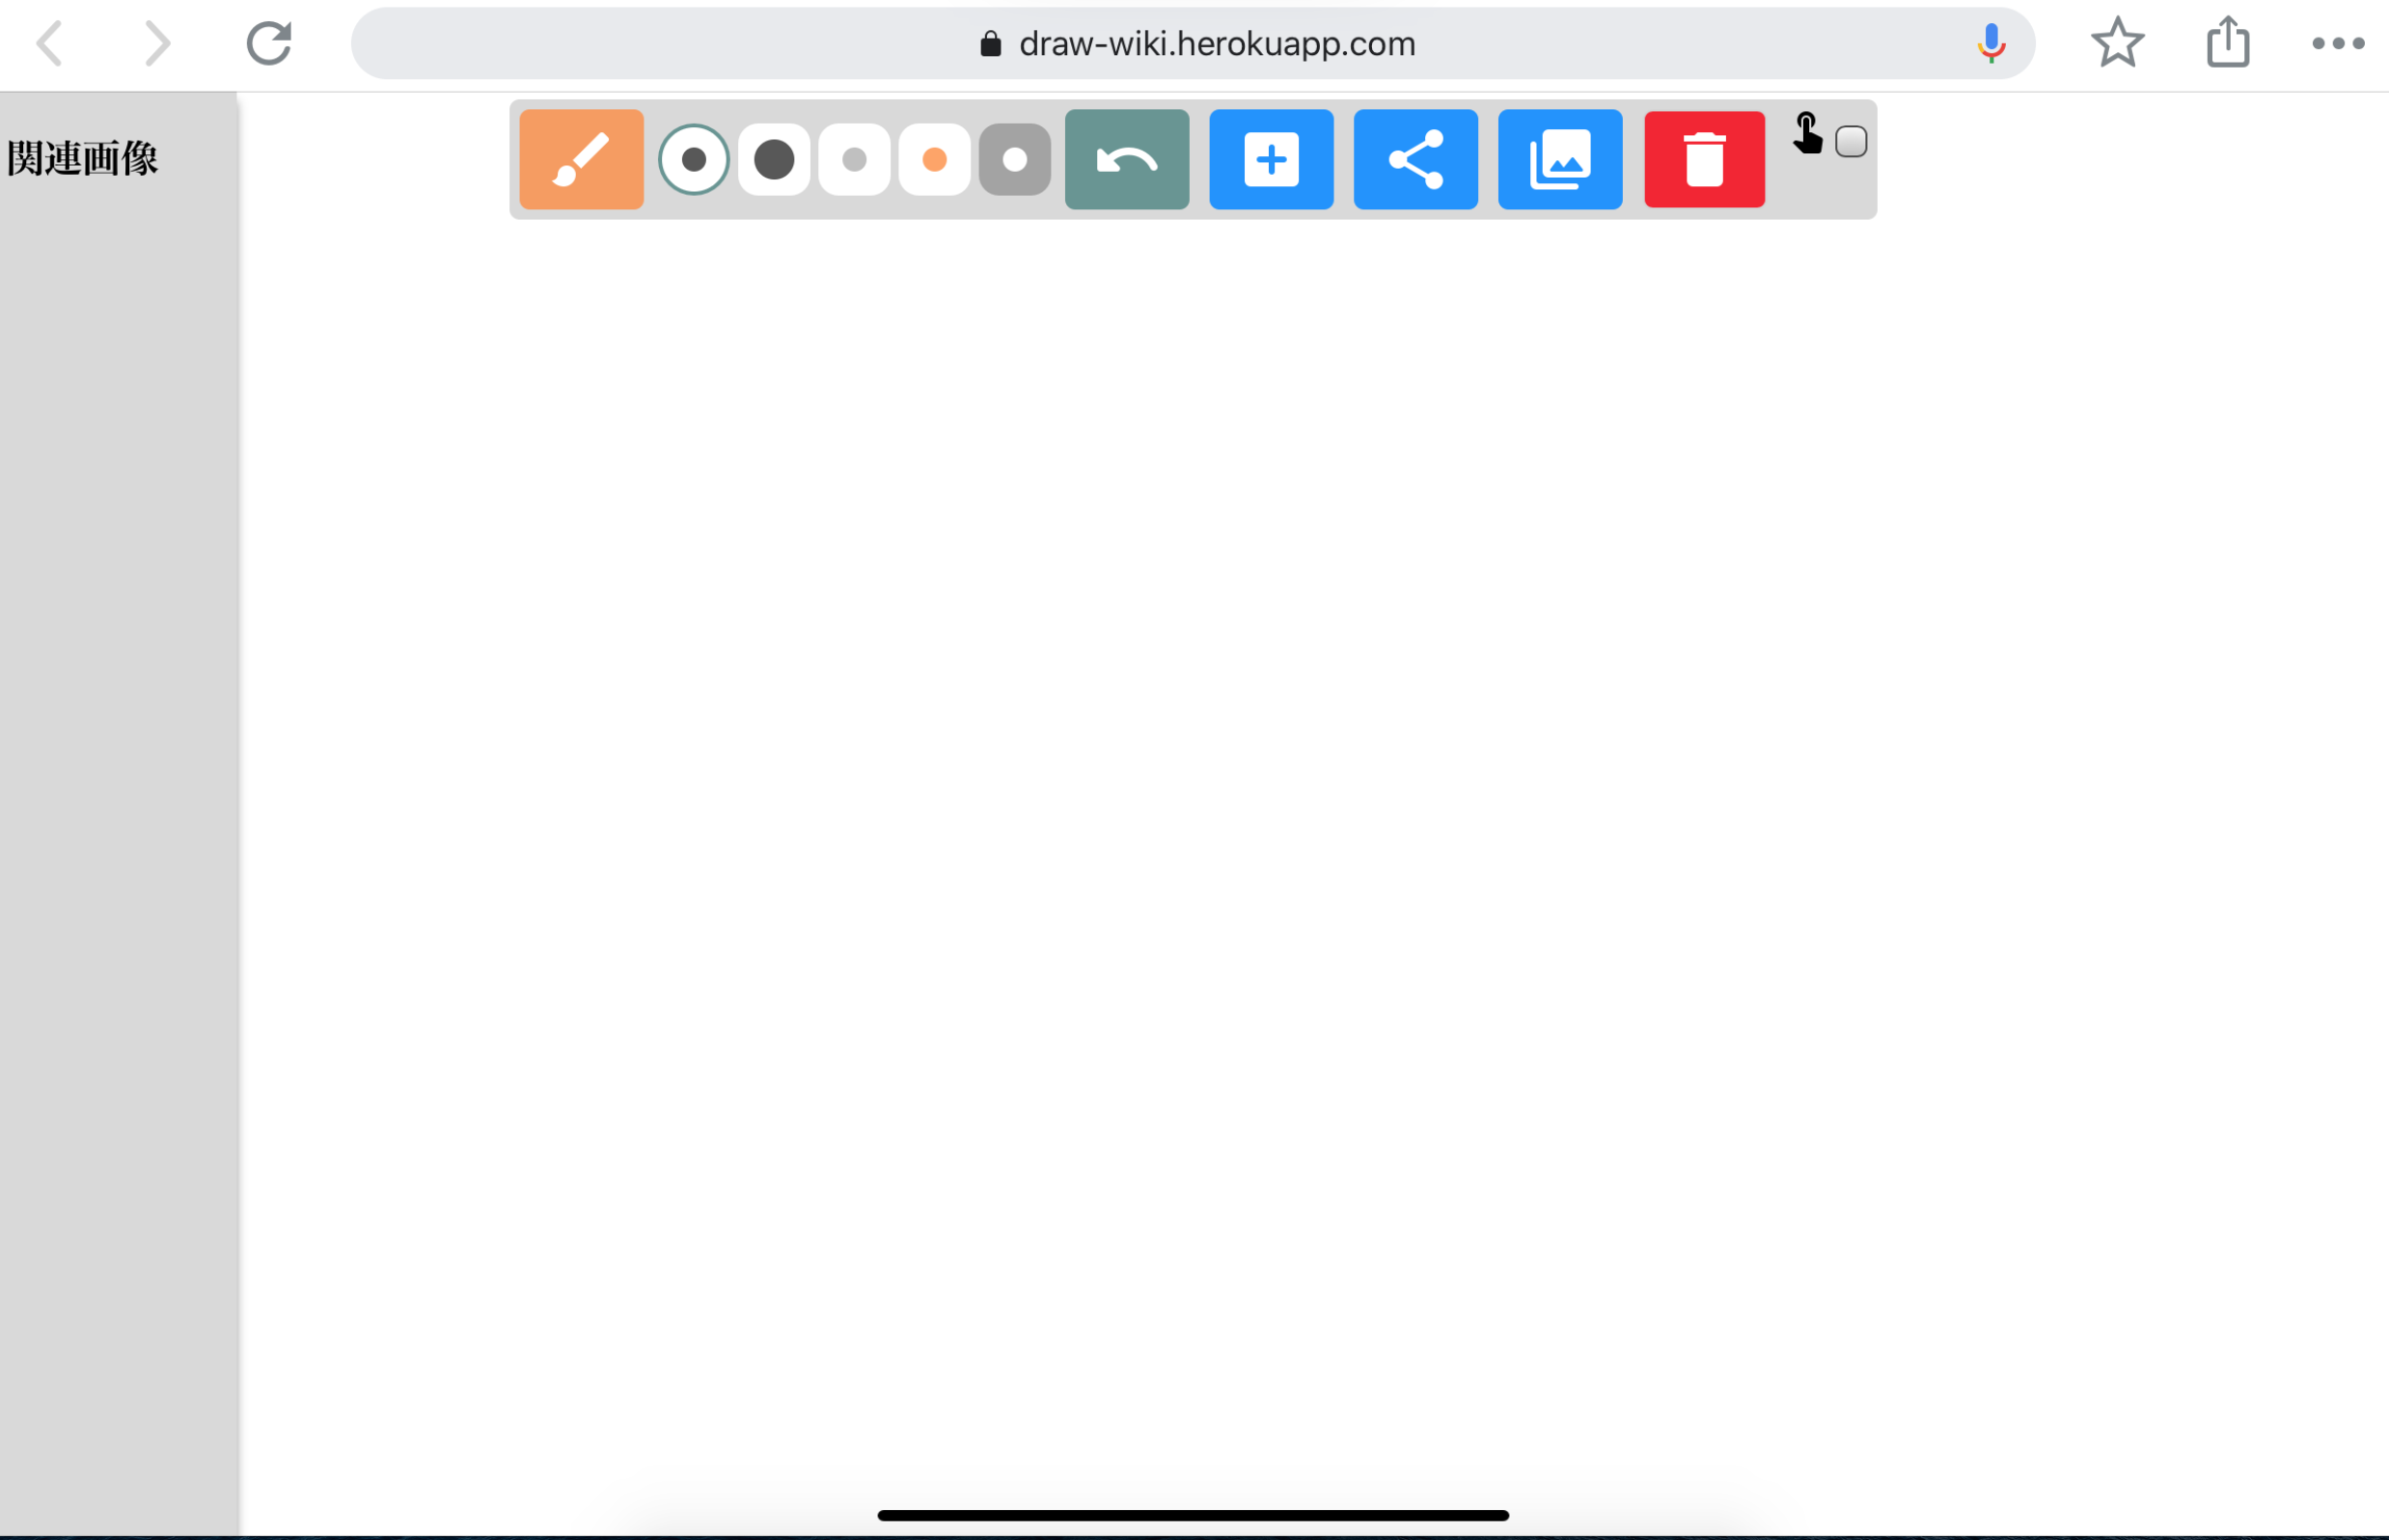
\includegraphics[width=70mm]{images/initialdrawwiki.png}} \end{center}
    \caption{DrawWikiの初期画面}
    \label{drawwiki}
\end{figure}

%\subsection{基本機能}
%手書きデータを扱う既存のエディタと同様に、DrawWikiはUndo・Redoやオブジェクトの変形・移動等、計算機によって実現可能になった便利な編集支援機能を備えている。
%これにより手軽に手書きメモ・イラストを作成することができる。
%
%\subsection{特有の機能と使い方}
%前章で述べた要件を満たすためにDrawWikiは特有の機能を備えている。使い方とともに解説する。

\subsection{機能と使い方}

%\paragraph*{ハイパーイラストの作成}
%画面中央部分に自由にイラストが描けるキャンバスを備えている。

\subsubsection{ハイパーリンクの作成・編集}

\begin{figure}[htbp]
    \begin{center}
        \fbox {
\includegraphics[width=80mm]{images/testimage.png}} \end{center}
    \caption{ハイパーイラストの作成画面}
    \label{hyperillustcreate}
\end{figure}
画面中央部分に自由に手書きができるキャンバスが配置されており、ここに描いたものが
ハイパーイラストとして自動的に保存・アップロードされる。
一度アップロードしたハイパーイラストには一意なURLが割り振られるため、
Webを通じて他のユーザーが閲覧し、また編集することもできる。

\subsubsection{ハイパーリンク埋め込み機能}

\begin{figure}[htbp]
    \begin{center}
        \fbox {
\includegraphics[width=80mm]{images/testimage.png}} \end{center}
    \caption{ハイパーリンク埋め込み機能の操作画面}
    \label{hyperlinking}
\end{figure}

範囲選択ツールを用いてハイパーリンクを埋め込みたい要素を選択することができる。
要素を選択して"他の図とリンクボタン"を押すと今まで作成したハイパーイラストのリストが開き、
その中からリンクさせたい図を選ぶとその図へのハイパーリンクが要素に埋め込まれる。

\subsubsection{関連するハイパーイラストの表示機能}

%\begin{figure}[htbp]
%%    \begin{center}
%%    {
\includegraphics[width=50mm]{images/testimage.png}} \end{center}
%%    \caption{関連イラストの表示機能}
%%    \label{linkedIllust}
%%\end{figure}

\begin{figure}[htbp] \begin{minipage}{0.5\hsize}
                         \begin{center} \fbox {
\includegraphics[width=70mm]{images/testimage.png}}
                         \end{center} \caption{関連イラストの表示機能} \label{fig:linkedIllust1}
\end{minipage} \begin{minipage}{0.5\hsize}
                   \begin{center} \fbox {
\includegraphics[width=70mm]{images/testimage.png}}
                   \end{center} \caption{関連イラストのモーダル} \label{fig:linkedIllust2}
\end{minipage}
\end{figure}

リンク機能を用いると、埋め込んだハイパーイラストのサムネイルがエディタの横の関連画像ビューに表示される。
このサムネイルを選択すると、そのイラストへのリンクが埋め込まれた要素が強調表示されるとともに、
そのイラストとリンクしている別のイラストをリストするモーダルが表示できる。
これによりイラスト同士のリンク関係が一目瞭然に理解でき、関連イラストを参照することができる。

%\subsubsection{ハイパーイラストのインポート機能}
%
%\begin{figure}[htbp]
%    \begin{center}
%    {
\includegraphics[width=50mm]{images/testimage.png}} \end{center}
%    \caption{インポート機能の操作画面}
%    \label{importing}
%\end{figure}
%
%過去に作成したハイパーイラストを一覧画面から選択し、現在編集中の画面にインポートすることができる。
%インポートした画像にも、元の画像へのハイパーリンクが含まれている。

\subsubsection{エキスポート・共有機能}

\begin{figure}[htbp]
    \begin{center}
    {
\includegraphics[width=50mm]{images/testimage.png}} \end{center}
    \caption{エキスポート機能の操作画面}
    \label{exporting}
\end{figure}

DrawWikiで作成したハイパーイラストには各々に一意なURLが割り振られており、どこからでも参照することができる。
また範囲選択ツールを用いて一部の範囲のみ別個のハイパーイラストとしてエキスポートすることができる。
本体のSVGは

\subsubsection{ブラシプリセット}
その他の特徴としてブラシのプリセットが金箱らによるInteractive Sketch\cite{130004638060}に基づいている。
%ラーナビリティの観点から機能を


\begin{figure}[htbp]
    \begin{center}
        \fbox {
\includegraphics[width=80mm]{images/testimage.png}} \end{center}
    \caption{プリセットを用いて描いた図}
    \label{interacive}
\end{figure}